\documentclass[10pt, a4paper]{scrartcl}

\usepackage{vorschule}
\usepackage[
    typ=ab,
    fach=Mathematik,
    lerngruppe={EF},
    nummer=8,
    module={Symbole,Lizenzen},
    seitenzahlen=keine,
    farbig,
    lizenz=cc-by-nc-sa-4,
]{schule}

\usepackage[
	kuerzel=Ngb,
	reihe={Differentialrechnung},
	version={2019-11-16},
]{ngbschule}

\author{J. Neugebauer}
\title{Motorradfahrt}
\date{\Heute}

\setzeAufgabentemplate{ngbnormal}

%\usepackage{qrcode}
%\usepackage{tinspire}


\begin{document}

\ReiheTitel

\begin{wrapfigure}{r}{0pt}
	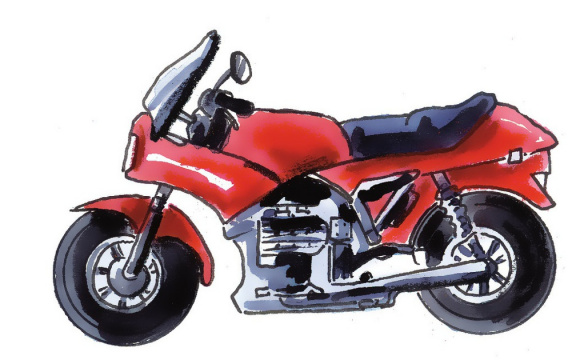
\includegraphics[width=4cm]{EF-AB.8-Abb_Motorrad}
%	\caption{Motorrad von Ute Ohlms}
\end{wrapfigure}

Thomas macht mit seinen Freunden am Wochenende eine Motorradtour. Während der Fahrt auf der Landstraße misst er seine zurückgelegte Strecke. Nach der Tour zeigt seine App an, dass für den gemessenen Teil der Tour (ca. \SI{5}{Stunden}) die zurückgelegte Strecke mit Hilfe der Funktion
\[ s(t) = -\frac{11}{16}\cdot t^4 + \frac{11}{4}\cdot t^3 + \frac{19}{4}\cdot  t^2 + 90\cdot t  \]
beschreiben wird ($t$ sind \si{Stunden}).

	
\begin{aufgabe}
	\begin{enumeratea}
		\item \operator{Zeichne} mit Hilfe des GTRs die Funktion und \operator{beschreibe} ihren Verlauf.
		\item \operator{Berechne} die durchschnittliche Änderungsrate in stündlichen Intervallen und \operator{interpretiere} diese im Sachzusammenhang.
	\end{enumeratea}
\end{aufgabe}

\begin{aufgabe}
	\SI{220}{Minuten}, nachdem er die Messung gestartet hat, wurde Thomas geblitzt. Er ist sich nicht sicher, ob er noch im Tolleranzbereich ($\SI{100}{\kilo\meter\per\hour} + \prozent{3}$) gefahren ist.

	\begin{enumeratea}
		\item \operator{Erkläre}, warum das Ergebnis der durchschnittlichen Änderungsrate nicht aussagekräftig ist, ob Thomas geblitzt wurde oder nicht.
		
		\item \operator{Berechne} die durchschnittliche Änderungsrate, die Thomas zwischen \num{3,5} und \SI{4}{Stunden}  hat. \operator{Erläutere}, warum auch dieser Wert noch keine Aussage zulässt, ob THomas zu schnell gefahren ist.
		
		\item Wie kann eine genauere Aussage über Thomas Geschwindigkeit zum Zeitpunkt der Radarkontrolle getroffen werden? \operator{Beschreibe} ein Verfahren, um eine Bessere Nährung der Geschwindigkeit zu erhalten. 
	\end{enumeratea}
\end{aufgabe}


\end{document}
